\section{Method}
\label{sec:method}

\begin{figure}[t]
  \centering
  \begin{subfigure}[b]{0.48\columnwidth}
    \centering
    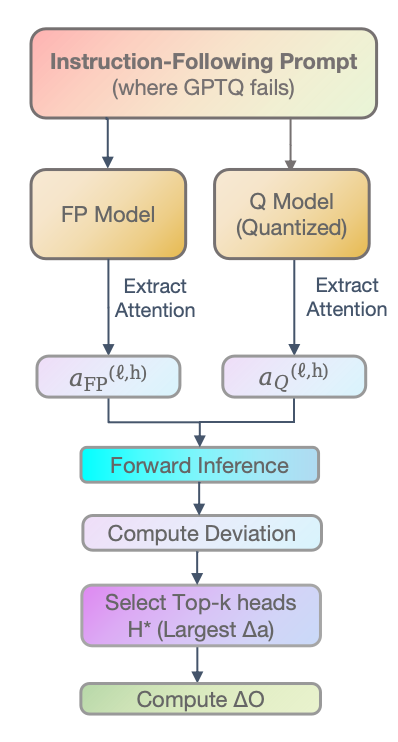
\includegraphics[width=\textwidth]{figures/figure2.png}
    \caption{Diagnostic phase}
    \label{fig:das_diagnostic}
  \end{subfigure}
  \hfill
  \begin{subfigure}[b]{0.5\columnwidth}
    \centering
    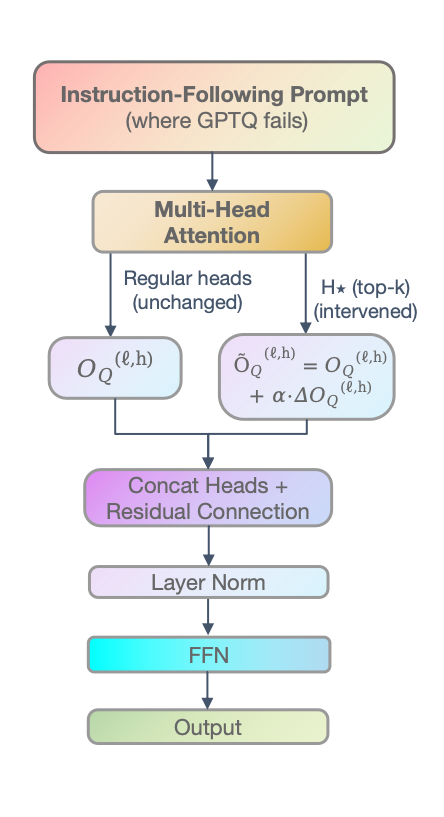
\includegraphics[width=\textwidth]{figures/figure2b.png}
    \caption{Intervention phase}
    \label{fig:das_intervention}
  \end{subfigure}
  \caption{\textbf{Overview of Deep Attention Stimulation (DAS).}
  \textbf{(a)} Comparing FP16 and quantized attention patterns identifies 
  degraded heads with reduced instruction token attention.
  \textbf{(b)} Inference applies $\alpha \cdot \Delta\mathbf{O}$ corrections 
  to these heads via forward hooks, restoring capability without retraining.}
  \label{fig:das_overview}
\end{figure}

\subsection{Problem Setup}

Let $\mathcal{M}_{\text{FP}}$ denote a full-precision instruction-tuned language
model and $\mathcal{M}_{\text{Q}}$ its post-training quantized counterpart (e.g.,
GPTQ-4bit).
Given a set of instruction-following prompts $\mathcal{D}$, we focus on
\emph{failure cases} where $\mathcal{M}_{\text{FP}}$ satisfies all instruction
constraints while $\mathcal{M}_{\text{Q}}$ violates at least one.
Our objective is to diagnose which internal attention heads are most affected by
quantization and to apply a training-free, inference-time intervention that
restores instruction-following behavior. Figure~\ref{fig:das_overview} illustrates the two-stage DAS framework.

\subsection{Locating Instruction-Bearing Tokens}

Instruction-following constraints are often explicitly stated in the prompt
(e.g., ``all lowercase'', ``no commas'', ``respond in English'').
For a prompt $x$, we approximate the \emph{instruction-bearing token set}
$\mathcal{I}(x)$ using lightweight heuristics such as keyword matching and
pattern rules.
This step provides a coarse localization of instruction-related tokens and does
not attempt to fully parse or interpret the instruction semantics.

\subsection{Head-Level Instruction Attention}
\label{sec:head_attention}

Consider a transformer layer $\ell \in \{1,\ldots,L\}$ and attention head
$h \in \{1,\ldots,H\}$.
Let $A^{(\ell,h)}_{\text{FP}}(x)$ and $A^{(\ell,h)}_{\text{Q}}(x)$ denote the
attention weight matrices (after softmax) produced by $\mathcal{M}_{\text{FP}}$
and $\mathcal{M}_{\text{Q}}$ on input $x$, respectively.
We quantify how strongly head $(\ell,h)$ attends to instruction-bearing tokens
by aggregating attention mass onto $\mathcal{I}(x)$:
\begin{equation}
a^{(\ell,h)}(x) =
\frac{1}{|\mathcal{T}(x)|}
\sum_{t \in \mathcal{T}(x)}
\sum_{i \in \mathcal{I}(x)}
A^{(\ell,h)}[t,i],
\label{eq:instruction_attention}
\end{equation}
where $\mathcal{T}(x)$ denotes all query token positions within the prompt and
generated sequence for input $x$.
For brevity, we omit the model subscript when the context is clear.

\subsection{Diagnosing Quantization-Induced Deviation}
\label{sec:diagnosis}

Let $\mathcal{F} \subset \mathcal{D}$ denote the set of instruction-following
failure cases.
We define the \emph{instruction-saliency deviation} of head $(\ell,h)$ as:
\begin{equation}
\Delta a^{(\ell,h)} =
\frac{1}{|\mathcal{F}|}
\sum_{x \in \mathcal{F}}
\left(
a^{(\ell,h)}_{\text{FP}}(x)
-
a^{(\ell,h)}_{\text{Q}}(x)
\right).
\label{eq:delta_attention}
\end{equation}

% Positive values indicate increased attention to instruction tokens after
% quantization, while negative values indicate suppression.
Positive values indicate reduced instruction attention under quantization, while negative values indicate amplification.
In this pilot study, we rank heads by the magnitude
$|\Delta a^{(\ell,h)}|$, capturing both amplification and attenuation effects
induced by quantization.
We then select the top-$k$ most affected heads:
\begin{equation}
\mathcal{H}^\star =
\text{Top-}k
\left(
\left\{
|\Delta a^{(\ell,h)}|
\right\}_{\ell,h}
\right).
\label{eq:critical_heads}
\end{equation}

\subsection{Deep Attention Stimulation}
\label{sec:das}

\paragraph{Correction target.}
We intervene at the level of individual attention head outputs, which allows
localized modification of model behavior without altering weights or retraining.

Let $O^{(\ell,h)}_{\text{FP}}(x)$ and $O^{(\ell,h)}_{\text{Q}}(x)$ denote the
context vectors produced by head $(\ell,h)$ at layer $\ell$ under the
full-precision and quantized models, respectively.
We define the per-head corrective signal as:
\begin{equation}
\Delta O^{(\ell,h)}(x)
=
O^{(\ell,h)}_{\text{FP}}(x)
-
O^{(\ell,h)}_{\text{Q}}(x).
\label{eq:delta_output}
\end{equation}

In our implementation, $\Delta O^{(\ell,h)}(x)$ is computed and cached per failure
sample during the diagnostic phase.

\paragraph{Inference-time intervention.}
During inference with the quantized model, DAS injects an $\alpha$-scaled
correction into the affected heads:

\begin{equation}
\begin{aligned}
\widetilde{O}^{(\ell,h)}(x) &= O^{(\ell,h)}_{\text{Q}}(x) + \alpha \cdot \Delta O^{(\ell,h)}(x), \\
&\qquad \forall\, (\ell,h) \in \mathcal{H}^\star.
\end{aligned}
\label{eq:das}
\end{equation}

This intervention is implemented using forward hooks in the attention module and
does not modify model parameters.
Heads not in $\mathcal{H}^\star$ remain unchanged.

\paragraph{Clarification of $\Delta O$ and Controlled Evaluation.}
In our current study, $\Delta O^{(\ell,h)}(x)$ is computed and applied
in a prompt-specific manner.
That is, for each diagnostic failure case $x$,
we cache the attention head output difference
between the full-precision and quantized models.
During inference, the corrective signal is applied
only when evaluating the same prompt $x$.
This design ensures that sequence length and token positions
match exactly between diagnosis and intervention,
allowing a clean before-and-after comparison
that isolates the effect of attention-level stimulation.

While this prompt-specific formulation does not generalize
to unseen inputs, it provides a controlled setting
for analyzing whether quantization-induced failures
can be repaired through targeted attention intervention.
Developing prompt-agnostic or averaged correction schemes
is left for future work.

\subsection{Algorithmic Summary}

Algorithm~\ref{alg:das} summarizes the complete DAS procedure.
The method consists of two stages:
(1) an offline diagnostic phase that identifies critical heads using a small set
of failure cases, and
(2) an online intervention phase that applies cached corrections during
inference with the quantized model.

% \begin{algorithm}[t]
% \caption{Deep Attention Stimulation (DAS)}
% \label{alg:das}
% \begin{algorithmic}[1]
% \Require Full-precision model $\mathcal{M}_{\text{FP}}$, quantized model
% $\mathcal{M}_{\text{Q}}$, prompts $\mathcal{D}$, number of heads $k$, strength
% $\alpha$
% \Ensure Inference with DAS corrections

% \State \textbf{// Offline Diagnostic Phase}
% \State Identify failure set $\mathcal{F} \subset \mathcal{D}$
% \For{each $x \in \mathcal{F}$}
%   \State Locate instruction tokens $\mathcal{I}(x)$
%   \State Extract attention matrices
%   $A^{(\ell,h)}_{\text{FP}}(x)$ and $A^{(\ell,h)}_{\text{Q}}(x)$
%   \State Compute $a^{(\ell,h)}(x)$ via Eq.~\eqref{eq:instruction_attention}
% \EndFor
% \State Compute $\Delta a^{(\ell,h)}$ via Eq.~\eqref{eq:delta_attention}
% \State Select critical heads $\mathcal{H}^\star$ via
% Eq.~\eqref{eq:critical_heads}
% \State Cache $\Delta O^{(\ell,h)}(x)$ for $(\ell,h)\in\mathcal{H}^\star$

% \State \textbf{// Online Intervention Phase}
% \For{each test prompt $x'$}
%   \State Run $\mathcal{M}_{\text{Q}}(x')$ with forward hooks enabled
%   \For{each $(\ell,h) \in \mathcal{H}^\star$}
%     \State Retrieve cached $\Delta O^{(\ell,h)}(x')$
%     \State Apply correction via Eq.~\eqref{eq:das}
%   \EndFor
%   \State Generate output with corrected activations
% \EndFor
% \end{algorithmic}
% \end{algorithm}

\begin{algorithm}[t]
\caption{Deep Attention Stimulation (DAS)}
\label{alg:das}
\begin{algorithmic}[1]
\Require Full-precision model $\mathcal{M}_{\text{FP}}$, quantized model
$\mathcal{M}_{\text{Q}}$, prompts $\mathcal{D}$, number of heads $k$, strength
$\alpha$
\Ensure Inference with DAS corrections (prompt-specific)

\State \textbf{// Offline Diagnostic Phase}
\State Identify failure set $\mathcal{F} \subset \mathcal{D}$ where $\mathcal{M}_{\text{FP}}$ passes and $\mathcal{M}_{\text{Q}}$ fails
\For{each $x \in \mathcal{F}$}
  \State Locate instruction tokens $\mathcal{I}(x)$
  \State Extract attention matrices $A^{(\ell,h)}_{\text{FP}}(x)$ and $A^{(\ell,h)}_{\text{Q}}(x)$
  \State Compute $a^{(\ell,h)}(x)$ via Eq.~\eqref{eq:instruction_attention}
\EndFor
\State Compute $\Delta a^{(\ell,h)}$ via Eq.~\eqref{eq:delta_attention}
\State Select critical heads $\mathcal{H}^\star$ via Eq.~\eqref{eq:critical_heads}
\For{each $x \in \mathcal{F}$}
  \State Cache $\Delta O^{(\ell,h)}(x)$ for all $(\ell,h)\in\mathcal{H}^\star$
\EndFor

\State \textbf{// Online Intervention Phase (controlled evaluation)}
\For{each prompt $x \in \mathcal{F}$} \Comment{current setup evaluates the same prompts as diagnosis}
  \State Run $\mathcal{M}_{\text{Q}}(x)$ with forward hooks enabled
  \For{each $(\ell,h) \in \mathcal{H}^\star$}
    \State Retrieve cached $\Delta O^{(\ell,h)}(x)$
    \State Apply correction via Eq.~\eqref{eq:das}
  \EndFor
  \State Generate output with corrected activations
\EndFor
\end{algorithmic}
\end{algorithm}
